\documentclass{article}

\usepackage[cm]{fullpage}
\usepackage{hyperref}
\usepackage{graphicx}
\usepackage{amsmath,amsfonts}

\begin{document}
\title{Uber exercises}
\author{Toby Dylan Hocking}
\maketitle

\section{Part 1: Data Analysis}

\subsection{Visualization of logins.json}

I used R and the RJSONIO package to read the logins.json file. There
are 93,142 times in the file, from 1970-01-01 20:13:18 to 1970-04-13
18:54:23. I used the data.table package to compute the total number of
logins in each 15-minute interval. There are 9788 intervals, some of
which have 0 logins. 

I used R and the ggplot2 and animint packages to create the following
interactive data visualization.

\url{http://cbio.ensmp.fr/~thocking/uber-exercise/figure-logins/}

One screenshot of the data viz is shown below.

\begin{center}
  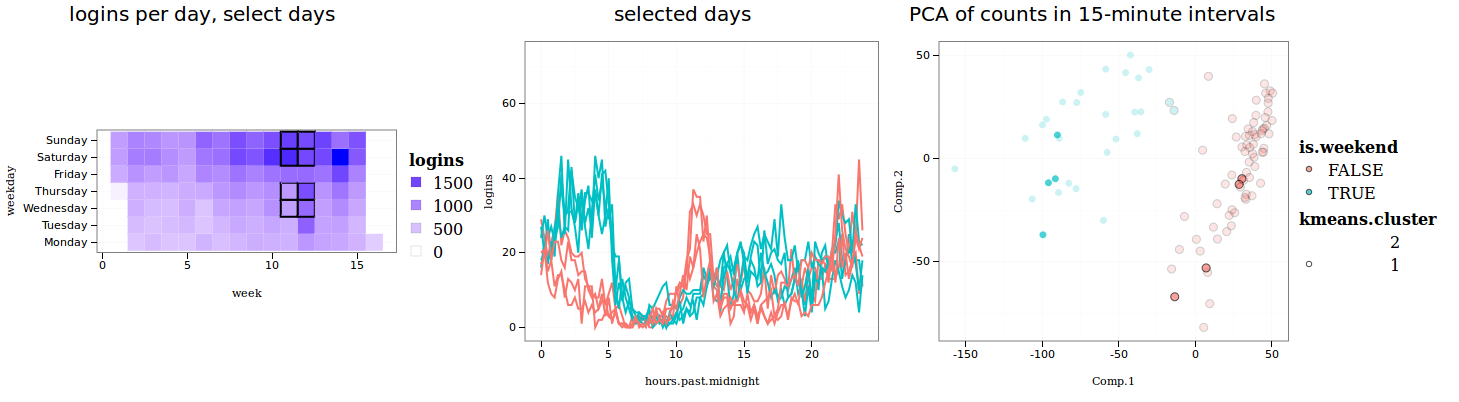
\includegraphics[width=\textwidth]{screenshot-viz-logins.png}
\end{center}

\begin{description}
\item[left plot] Clicking rectangles will select or de-select
  days. The rectangle fill color represents the total number of logins
  in that day (darker for more logins).
\item[middle plot] Login counts in each 15 minute interval are shown
  for the selected days (including intervals with 0 counts). The line
  color shows whether or not the data occur on a weekend (teal for
  Saturday or Sunday, orange for weekdays).
\item[right plot] Clicking points will select or de-select days. The
  PCA was computed by treating the counts for each day as a
  96-dimensional feature vector. The first and last days do not appear
  on the PCA plot because they did not have observations for all 96
  time intervals (103 days overall, 101 points plotted). The $k$-means
  algorithm was run with $k=2$ to find two clusters that best
  represent the 96-dimensional feature vectors, and the cluster labels
  are shown using the point border (black for cluster 1, white for
  cluster 2).
\end{description}

Overall it is clear from this data visualization that there are very
different patterns for weekends and weekdays. For example, weekends
tend to have lots more logins before 6am and in the afternoon, and
weekdays have lots more logins around noon (lunch time).

\subsection{Predictive model for the next four 15-minute intervals}

Since the quantity we want to predict is a count, the Poisson
regression model is appropriate. For every 15-minute interval $i$, we
have the actual number of logins $y_i\in\mathbb Z_+$ (a non-negative
integer), and we can compute $p$ numeric input features
$\mathbf x_i\in\mathbb R^p$ based on the time of day, day of the week,
counts in previous times, etc. The Poisson regression models each
login count via $y_i \sim \text{Poisson}(\lambda_i)$ with the Poisson
mean $\lambda_i = f(\mathbf x_i)$.

For accurate prediction, it is extremely important to use a
\textbf{regularized} Poisson regression, so that un-informative input
features in $\mathbf x_i$ will be ignored. I used
\texttt{glmnet::cv.glmnet(family="poisson")}, which implements
L1-regularization for the Poisson regression model.

To evaluate the accuracy of the model predictions, I divided the data
set into two sets:
\begin{description}
\item[train] the first 5000 intervals, approximately up to and
  including week 8 (the last day with all train intervals is
  1970-02-22).
\item[test] the rest of the data, approximately week 9 and after (the
  first test interval is on 1970-02-23).
\end{description}
I fit four separate regularized Poisson regression models to the same
$4777\times 31$ train feature matrix, using the four different outputs
(predict next 15-minute interval, the one after, etc).

I used \texttt{predict(type="response")} to get the predicted mean
parameters $\lambda_i$ for each interval in both the train and test
sets. Then I used \texttt{qpois(0.5, $\lambda_i$)} to get the
predicted median, which I would use for predicting the number of
logins (it is guaranteed to be a non-negative integer). I created the
following interactive data viz to qualitatively evaluate these predictions.

\url{http://cbio.ensmp.fr/~thocking/uber-exercise/figure-poisson-model/}

One screenshot from this data viz is shown below:

\begin{center}
  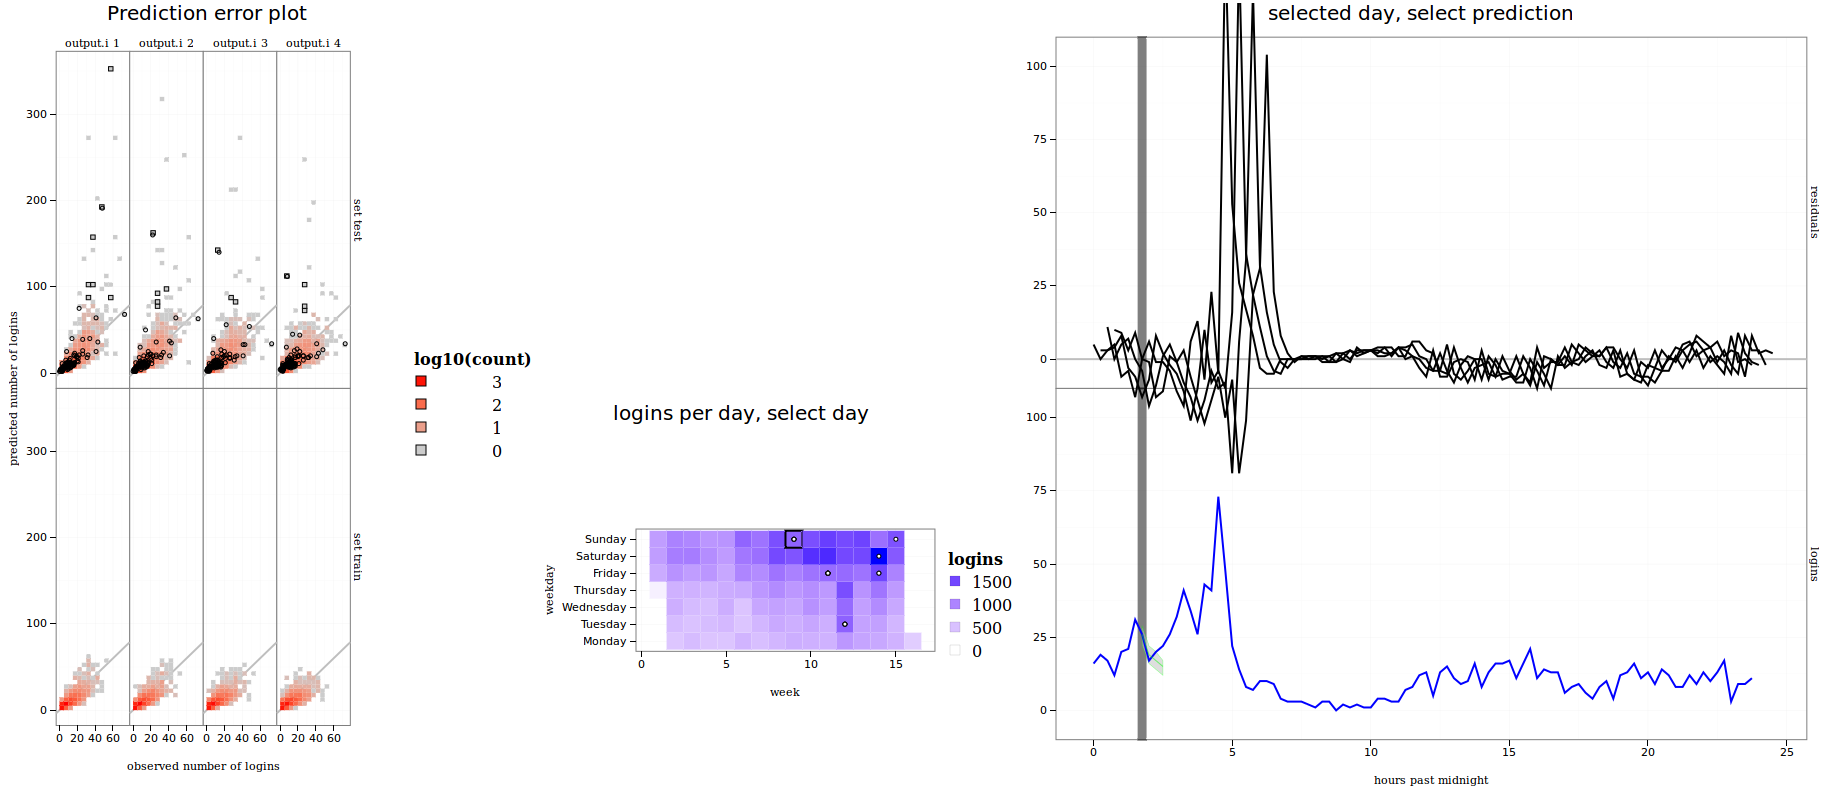
\includegraphics[width=\textwidth]{screenshot-predictions.png}
\end{center}

\begin{description}
\item[left plot] Scatterplots show predicted number of logins as a
  function of the observed number of logins, with panels for
  train/test sets and each of the 4 prediction problems. The fill
  color shows the number of predictions in each rectangle (dark red
  for more predictions). It is clear that the vast majority of the
  model predictions occur along the predicted=observed line (grey
  diagonal line). It is also clear that there are a few test
  predictions for which the model predicts too many logins. Black
  points are drawn for the predictions of the currently selected day.
\item[middle plot] Clicking a rectangle selects that day. White points
  are drawn for days which include the rectangles which have been
  clicked in the first plot.
\item[right plot] Details of login counts (blue) and model residuals
  (black) are shown for the selected day. Predictions for the next
  four time points are shown as a green line with a grey confidence
  band. The animation advances the time point for predictions, and
  clicking the background can also change the prediction that is
  shown. It is clear that the big prediction errors usually happen
  around spikes in the data.
\end{description}

To quantitatively compare this model with some alternative model
(perhaps a non-linear model such as K-nearest-neighbors), we could
compute the mean squared prediction error (MSE) with respect to all test
data. Say that $g:\mathbb R^p\rightarrow \mathbb Z_+^4$ is a function
that gives the predictions in the next four time intervals. We can
evaluate it by computing
\begin{equation}
  \text{MSE}(g) = \sum_{i\in\text{test}} ||g(\mathbf x_i)-\mathbf y_{i}||^2_2,
\end{equation}
where $\mathbf y_i\in\mathbb Z_+^4$ is the vector of observed counts
in the times after $i$, and $||\cdot||_2^2$ is the squared 2-norm (sum
of squares of elements of the vector). If we have two candidate
prediction functions $g_1$ and $g_2$ with
$\text{MSE}(g_1)<\text{MSE}(g_2)$ then we can conclude that $g_1$ is
better for prediction.

More generally, this method is limited by the definition of the input
features $\mathbf x_i$, which must be done by a human. So actually a
human must do some manual pattern recognition to determine which
features to compute for the model. In the future it would be
preferable to use another model which does not depend on human
learning. For example, the spectral mixture kernel is a Bayesian
non-parametric forecasting method that does not need manual feature or
kernel engineering:

\url{https://arxiv.org/abs/1302.4245}

\subsection{Stochastic predictions}

The Poisson regression model inherently models the stochastic nature
of the prediction. To get a predicted confidence band around the
median, I used \texttt{qpois(0.25, $\lambda_i$)} to get the predicted
lower quartile, and \texttt{qpois(0.75, $\lambda_i$)} to get the
predicted upper quartile. Both of these quantities are guaranteed to
be non-negative integers, and I used them to draw the green confidence
band in the last panel of the interactive data viz.

To quantitatively evaluating these stochastic predictions, one could
compute the fraction of test outputs that fall within the predicted
confidence band. Since this is the inter-quartile range, we would
expect one-half of the data points to fall in the range. If there are
two different methods for computing 50\% confidence bands, then we
should prefer whichever gets closer to that quantity empirically on
the test set.

\section{Appendix: source code}

\url{https://github.com/tdhock/uber-exercise}

\end{document}
